
\section{Non-linear transformations}

\begin{frame}\frametitle{\secname}

\only<1>{
\notesonly{We use $N$ to denote the dimensionality of our input space and $p$ to denote the number of observations.\\}
Let $\vec x^{(\alpha)} \in \R^N$ and $\alpha = 1, \ldots, p$.

\notesonly{The following} mapping\notesonly{ describes the non-linear transformation of each observation}:
\svspace{-3mm}
\begin{equation}
\vec{\phi}: \vec{x} \mapsto \vec{\phi}_{(\vec{x})}
\end{equation}

}
\only<1->{
\notesonly{An e}\slidesonly{E}xample\notesonly{ of such a transformation }- 2\textsuperscript{nd}-order monomials:
\begin{equation}
\vec{\phi}_{(\vec{x})} = ( 
    1, \;
    \mathrm{x}_1, \;
    \mathrm{x}_2, \;
    \ldots \;
    \mathrm{x}_N, \;
    \mathrm{x}_1^2, \; 
    \mathrm{x}_1 \mathrm{x}_2, \;
    \mathrm{x}_2^2, \;
    \mathrm{x}_1 \mathrm{x}_3, \;
    \mathrm{x}_2 \mathrm{x}_3, \;
    \mathrm{x}_3^2, \; \ldots, \;
    \mathrm{x}_N^2
    )^\top
\end{equation}

\svspace{-5mm}
\begin{center}
\only<2>{
	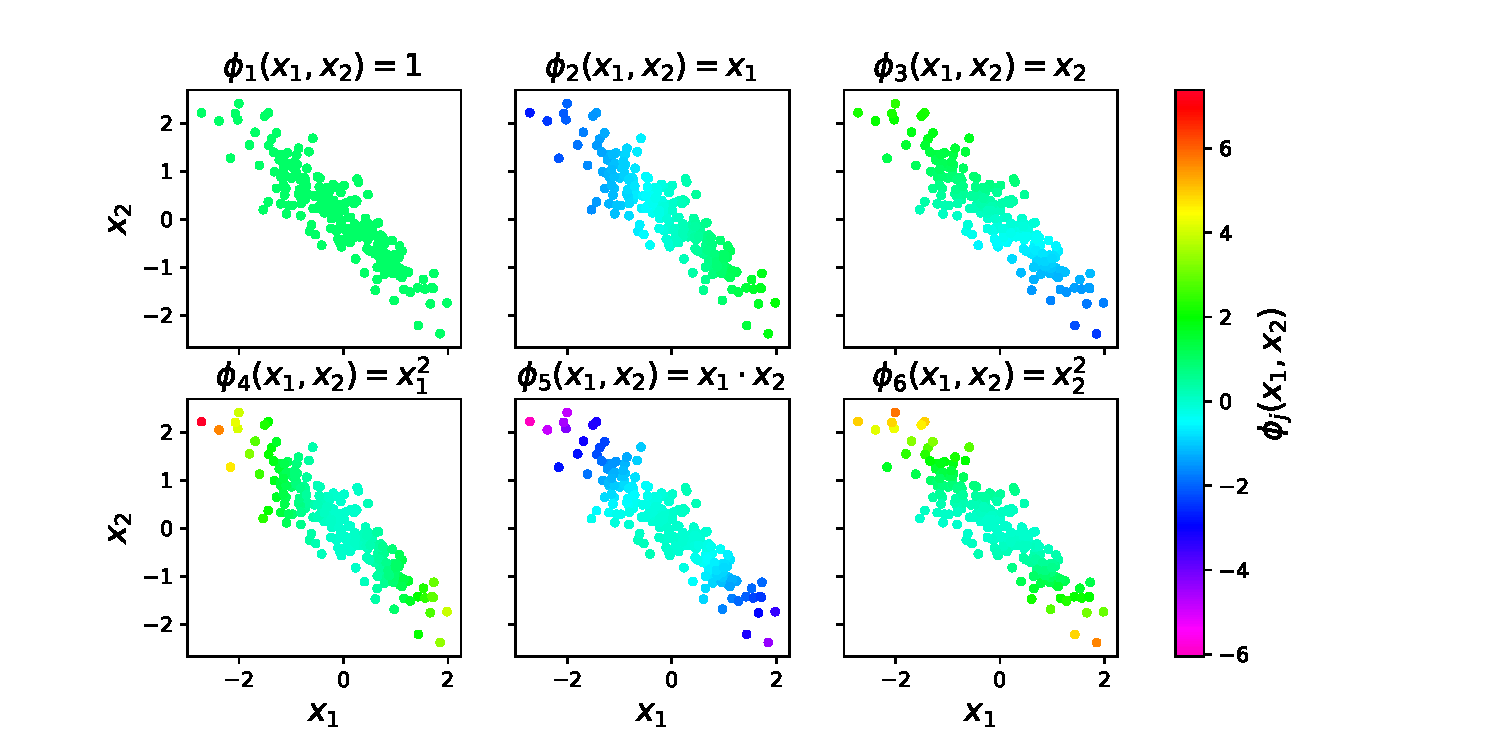
\includegraphics[width=0.87\textwidth]{img/monomials}%
	}
	\only<3>{
	\slidesonly{
		
\includegraphics[width=0.7\textwidth]{img/meme_candononlinpca}%
	}
	}
	\mode<article>{
	\captionof{figure}{Monomials for 2-d input}
	}
\end{center}
}
\only<2->{
\svspace{-5mm}
We could perform PCA on the transformed data $\vec \phi_{(\vec x)}$.\\
\notesonly{The reasoning behind this is that }non-linear correlations between variables in $\vec x$ could be linear between variables in $\vec \phi_{(\vec x)}$.

\notesonly{
This is the \underline{purpose} of the non-linear transformaiton. That, two or more components in the original $\vec x$ (e.g. $x_1$, $x_2$) could have non-linear correlations (e.g. plotting those two components reveals a parabola). 
Expanding the dimensionality of $\vec x$ through the above mapping introduces new dimensions in which correlations between the components in $\vec \phi_{(\vec x)}$ become \emph{linear}.

}
}

\end{frame}

\begin{frame}\frametitle{\secname}

\pause
\notesonly{However,} we might not know how to define $\vec \phi_{(\vec x)}$.

\pause

The potentially very high dimensionality of $\vec \phi_{(\vec x)}$ could prohibit us from storing the transformed data.\\

\begin{center}
	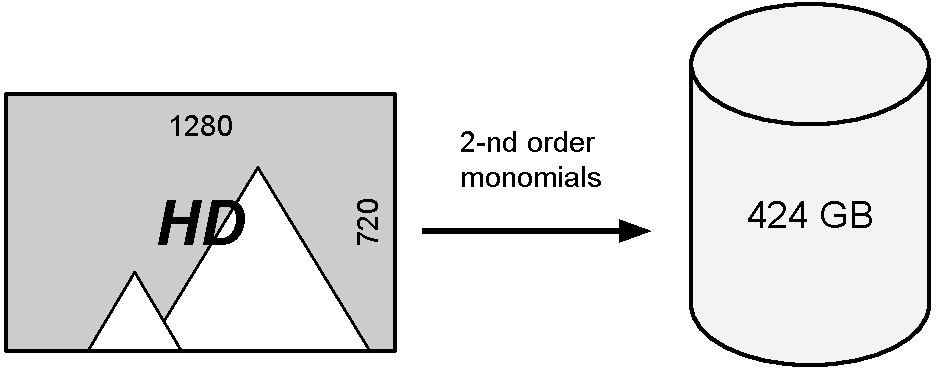
\includegraphics[width=0.5\textwidth]{img/storehd}%
	\notesonly{
	\captionof{figure}{Storing 2-nd order monomials applied to an HD image.}
	}
\end{center}

\notesonly{
2-nd order monomial applied to one HD ($1280 \times 720$ pixels) image would require more than $400 GB$ of storage alone\footnote{
$N=1280 \times 720 = 921600$ pixels, $d = \# x^1_j + \# x^2_j + \# \binom{N}{2} = (N+1) + N + \binom{N}{2} = 424,674,662,401$\\
Let's say it's a grayscale image, so 1 Byte per pixel. This way we end up with $424$ GB and some change.
}
}


\pause

\svspace{5mm}

\textbf{Caveat}:\\
Directly applying this transformation on a single observation is not applicable. 
We might never find a transformation that causes all non-linear correlations within $\vec x$ to become linear.\\

\end{frame}

\begin{frame}\frametitle{\secname}

The upside:\\

We actually don't need to define this transformation.
All we need to know is that the dimensionality of $\vec{\phi}_{(\vec{x})}$ can be larger than $N$, possibly infinitely large.\\

We turn to the ``kernel trick'' to solve this problem and avoid an epxlicit definition for the non-linear transformation.

\end{frame}
